\documentclass[10pt,a4paper]{article}
\usepackage[total={18cm,21cm},centering, headsep = 20pt, showframe=false]{geometry}
\usepackage[utf8]{inputenc}
\usepackage[spanish]{babel}
\usepackage{amsmath}
\usepackage{amsfonts}
\usepackage{amssymb}
\usepackage{mathrsfs}
\usepackage{float}
\usepackage{hyperref}

\usepackage{wrapfig}
\usepackage{graphicx}
\usepackage{pstricks}



% Default fixed font does not support bold face
\DeclareFixedFont{\ttb}{T1}{txtt}{bx}{n}{8} % for bold
\DeclareFixedFont{\ttm}{T1}{txtt}{m}{n}{8}  % for normal

% Custom colors
\usepackage{color}
\definecolor{deepblue}{rgb}{0,0,0.5}
\definecolor{deepred}{rgb}{0.6,0,0}
\definecolor{deepgreen}{rgb}{0,0.5,0}

\usepackage{listings}

% Python style for highlighting
\newcommand\pythonstyle{\lstset{
language=Python,
basicstyle=\ttm,
morekeywords={self},              % Add keywords here
keywordstyle=\ttb\color{deepblue},
emph={MyClass,__init__},          % Custom highlighting
emphstyle=\ttb\color{deepred},    % Custom highlighting style
stringstyle=\color{deepgreen},
frame=tb,                         % Any extra options here
showstringspaces=false
}}


% Python environment
\lstnewenvironment{python}[1][]
{
\pythonstyle
\lstset{#1}
}
{}

% Python for external files
\newcommand\pythonexternal[2][]{{
\pythonstyle
\lstinputlisting[#1]{#2}}}

% Python for inline
\newcommand\pythoninline[1]{{\pythonstyle\lstinline!#1!}}

\author{Ángel Edmundo Hernández Martínez}
\title{Reporte Técnico de Servicio Social.}
\date{}

\begin{document}

\maketitle

\section{Introducción}

	El siguiente documento es producto de mi Servicio Social en el Instituto de Investigaciones Económicas de la UNAM, bajo la asesoría directa del Dr. Gustavo Carreón Vázquez, durante el periodo que comprende el 18 de abril del 2022 al 17 de noviembre del 2022. \\
	
	El proyecto desarrollado durante el servicio social consta de los siguientes scripts, 
	
\begin{itemize}
	
	\item[•] \textit{Ecuacionlogistica.py}, en donde se desarrollan distintas funciones respecto a la ecuación logística, como su graficación, calcular sus datos y almacenarlos en formato .scv.
	
	\item[•] Diagrama_bifurcacion.py, en donde se grafica el diagrama de bifurcación de la ecuación logística.
	
	\item[•] Data_extraction.py, en donde se extraen los datos de distintos índices económicos y se almacenan en archivos scv.
	
\end{itemize}

	A continuación será explicado con mayor profundidad el funcionamiento de dichos scripts.
	
\section{Ecuación logistica y la complejidad}

	Para familiarizarnos con el estudio de la complejidad y el caos tratamos el caso de la Ecuación Logística. 
	La ecuación logística es un modelo de crecimiento poblacional publicado por Pierre Verhulst. Que se expresa con la siguiente ecuación iterativa;
	
	\begin{align*}
	x_{t+1} =  r\cdot x_{t}(1 - x_t), \text{ donde } 0 \leq x_0 \leq 1 
	\end{align*}
	
	La ecuación puede ser interpretada como la evolución de una población a lo largo del tiempo en la que la población máxima es $M = 1$ y las $x_t$ son fracciones de población. Es decir, que $x_t = \frac{1}{2}$, quiere decir que la población será $P_n = \frac{M}{2}$, por consiguiente $x_t$ sólo puede tomar valores comprendidos entre $0$ y $1$.\\
		
	 Otra cosa que es necesario tomar en cuenta es que para que la ecuación, en efecto, represente un modelo de evolución de poblaciones la constante $r$ no puede tomar un valor cualquiera. Veremos a continuación que los valores admisibles de $r$  están comprendidos entre $0$ y $4$.\\	
	 
	 Como las $x_t$ no pueden tomar valores negativos ni mayores a $1$, entonces,
	 
	 \begin{align*}
	 & 0 \leq x_{t+1} = r\cdot x_t(1-x_t) \leq 1 \\
	 \Rightarrow \hspace{.2cm} & 0 \leq x_t(1-x_t) \leq \frac{1}{r}
	 \end{align*}
	 
	 Luego, como la función $x_t(1-x_t)$ alcanza su valor máximo cuando $x_t = \frac{1}{2}$, tenemos,
	 
	 \begin{align*}
	 x_t(1-x_t) \leq \frac{1}{2}(1 - \frac{1}{2}) = \frac{1}{4} \leq \frac{1}{r}
	 \end{align*}
		
	En realidad, hemos calculado el máximo absoluto de la función $y = r\cdot x (1 - x)$ en el intervalo $[0,1]$. La función se anula en los extremos del intervalo, luego el valor máximo lo alcanza en el valor de $x$ que verifica: $y' = -2x + 1 = 0$. Es decir, $x = \frac{1}{2}$. Por lo tanto, los valores admisibles de $r$ están comprendidos entre $0$ y $4$, ambos incluidos.\\
	
	A continuación, explicaremos la función de \textit{Ecuacionlogistica.py} y veremos el comportamiento de la ecuación logística según algunos valores de $r$.Pues bien, en primer lugar importamos las distintas librerias  que ocuparemos, 	
	
\begin{python}
import math
import statistics
import numpy as np 
import matplotlib.pyplot as plt 
from random import randint 
import pandas as pd 
import seaborn as sns
\end{python}

	El módulo \pythoninline{seaborn} sirve para generar gráficas más elegantes 
	
	La función \pythoninline{logistic} tiene los siguientes parámetros:
	
	\begin{itemize}
	\item[•] \pythoninline{R} \* Se trata de la constante $r$ de la ecuación logísitica. En donde, para que tenga sentido, debe tomar valores en el intervalo $[0,4]$.
	\item[•] \pythoninline{x0} \* Es el valor inicial con el se comenzará a evaluar la ecuación logística, y como mencionamos se debe cumplir que $0 \leq x_0 \leq 1$.
	\item[•] \pythoninline{N} \* Es la cantidad de iteraciones de la ecuación logística.
	\end{itemize}
	
	La salida de la función es,
	
	\begin{itemize}
	\item[•] \pythoninline{x_list} \* Una lista con los valores obtenidos de haber usado iterativamente la ecuación logística
	\item[•] \pythoninline{R} \* La constante $r$ de la ecuación logística.
	\item[•] \pythoninline{x0} \* El valor inicial con el que empezamos la iteración de la ecuación logística. 
	\end{itemize}
		
\begin{python}
def logistic (R, x0, N):
    x = x0
    x_list = [x0]
    for i in range(N-1):
        x = R * x * (1.0 - x)
        x_list.append(x)

    return x_list, R, x0
\end{python}

A continuación, explicamos la función \pythoninline{graficar}. Sus parámetros son, 

\begin{itemize}
\item[•] \pythoninline{x_list} \hspace{.2cm} La lista con los valores de aplicar reiteradamente la ecuación logística. 
\item[•] \pythoninline{R} \hspace{.2cm} Es el parámetro $r$ de la ecuación logística.
\item[•] \pythoninline{x0} \hspace{.2cm} El valor inicial $x_0$ de la ecuación logística. 
\end{itemize}

La función obtiene una gráfica con los valores especificados de la ecuación logística, además de que guarda la gráfica obtenida en el mismo directorio.

\begin{python}
def graficar(x_list, R, x0):
    plt.style.use('seaborn-whitegrid')
    plt.figure(figsize=(16, 6), facecolor='lightgray')
    plt.xlabel('Numero de iteraciones')
    plt.ylabel('Valor de x')
    plt.title(f'\nEcuacion logistica\n\nR={R}  |  x0={x0}\n')
    plt.plot(x_list, 'o:r')
    plt.show()
    if (png_counter != 0):
        plt.savefig(f'Ecuacion logistica_{png_counter}.png')
\end{python}

Al estudiar la evolución en el tiempo de una población gobernada por la ecuación logística, para algunos valores de $r$ se observa un fenómeno interesante: la población alcanza un determinado valor, digamos $a$, y, a partir de ese valor permanece fijo en sucesivas generaciones. En este caso, tendriamos que $x_{t+1} = x_t =  a$, y de ahí que;

\begin{align*}
& a = r \cdot a (1 - a) \\
\Rightarrow \hspace{.2cm} &  0 = r a - r a^2 - a \\
\Rightarrow \hspace{.2cm} & 0 = a(r - 1) - r a^2 \\
\Rightarrow \hspace{.2cm} & 0 = a [(r - 1) - r a] \\
\Rightarrow \hspace{.2cm} & a = 0 \text{ y } a = \frac{r - 1}{r}
\end{align*}

Es decir, que la población alcanza un punto fijo cuando adquiere cualquiera de los dos valores anteriores. Pero, la ecuación logística presenta comportamiento diferente según los valores de la constante $r$. A continuación, exponemos las siguientes situaciones:

\begin{itemize}
\item[1.] Cuando $0 \leq r \leq 1$, independiente del valor inicial $P_0$ del que partamos, la población tiende asintóticamente a cero, es decir, que la población se extinguirá en unas pocas generaciones. 

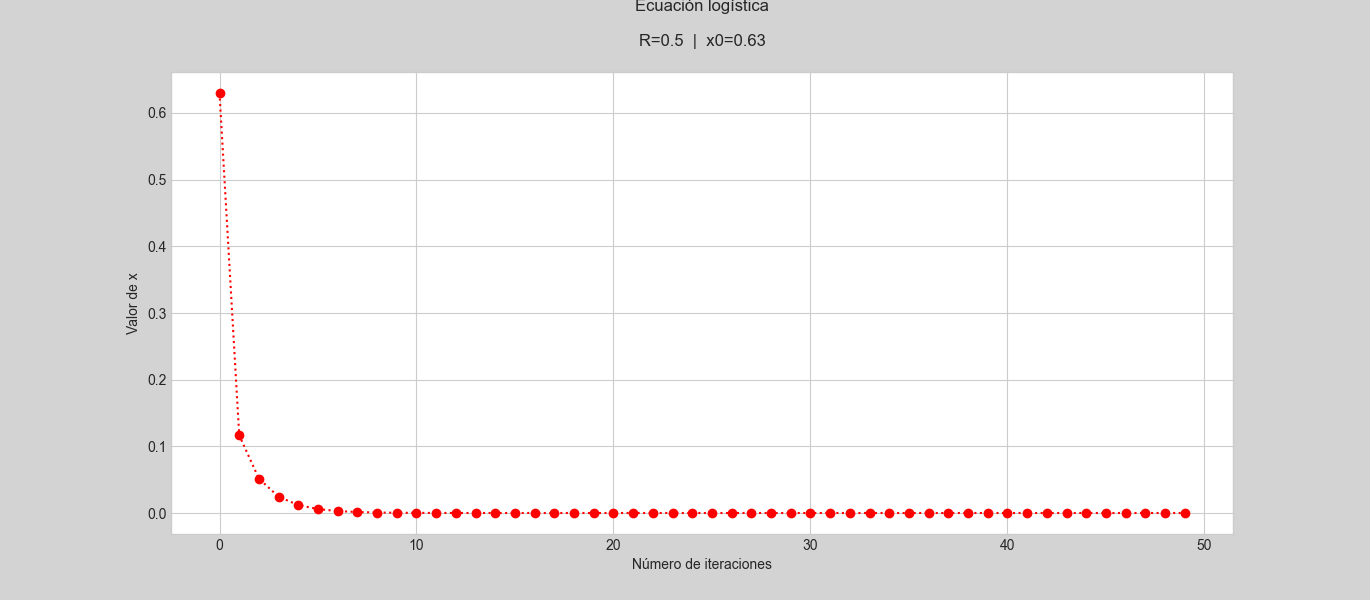
\includegraphics[scale=0.5]{Graf_1.png} 

\item[2.] Para $1 \leq r < 3$ se observa que la población tiende al punto fijo $\frac{r-1}{r}$, con independencia del valor inical que tomemos.

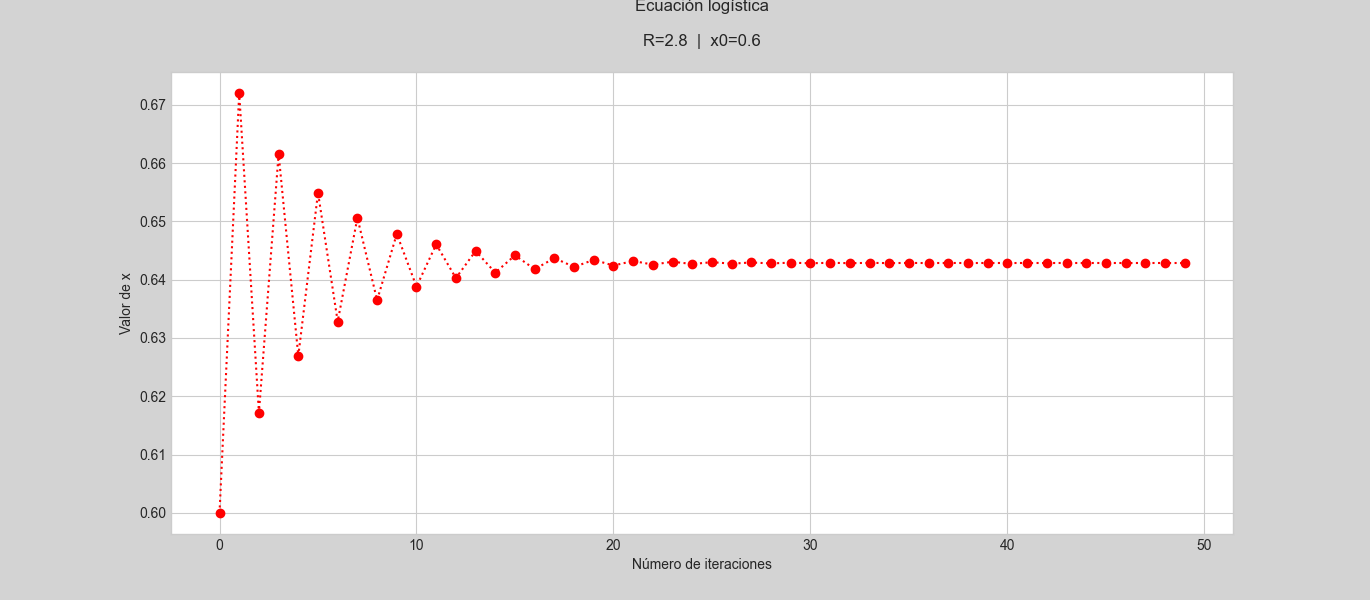
\includegraphics[scale=0.5]{Graf_2.png} 

\item[3.] Cuando $3 \leq r < 3.449$ el punto fijo se vuelve inestable y la población oscila alternativamente entre dos valores fijos estables, como se observa en la gráfica siguiente:

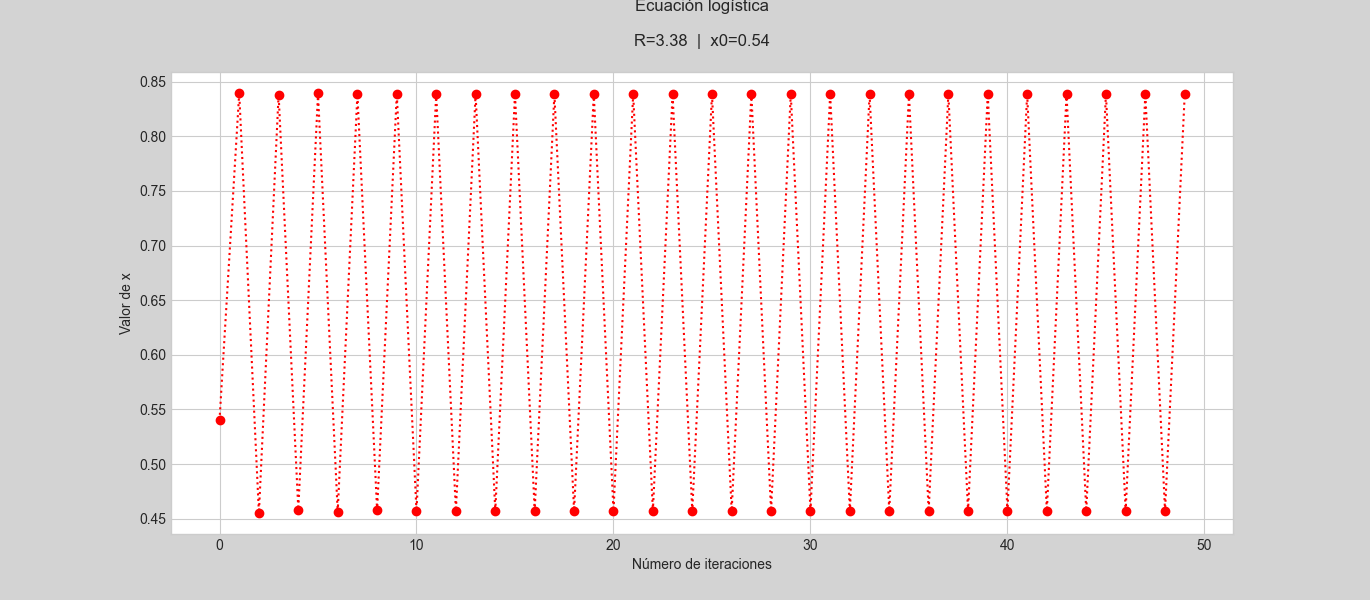
\includegraphics[scale=0.5]{Graf_3.png} 

\item[4.] Cuando $3.449 < r < 3.56994546$, se observa que la población final oscila entre cuatro, ocho, dieciséis, ..., o $2^n$ valores, presentando la gráfica aspectos como el siguiente, que oscila entre 4 valores,

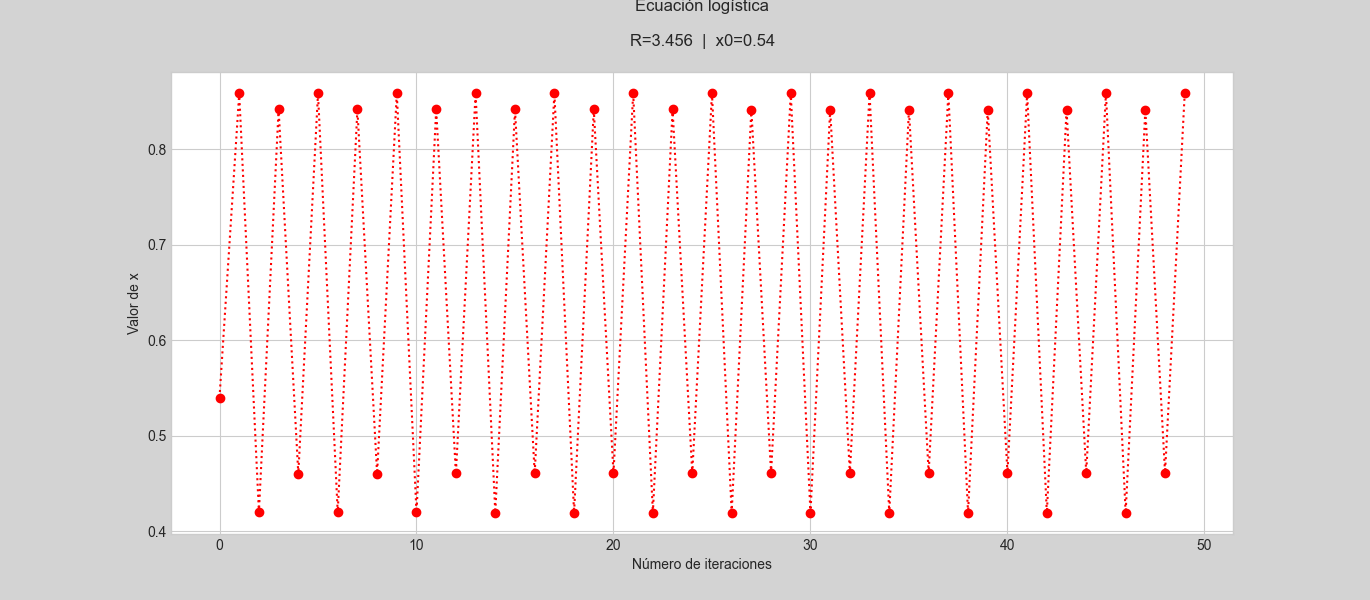
\includegraphics[scale=0.5]{Graf_4.png} 

\item[5.] Cuando $3.56994546 < r < 4$ aparece le comportamiento caótico. Y la gráfica oscila de forma irregular e imprevisible y dependiendo del valor inicial con el que se inicia la iteración, como en la siguiente gráfica:

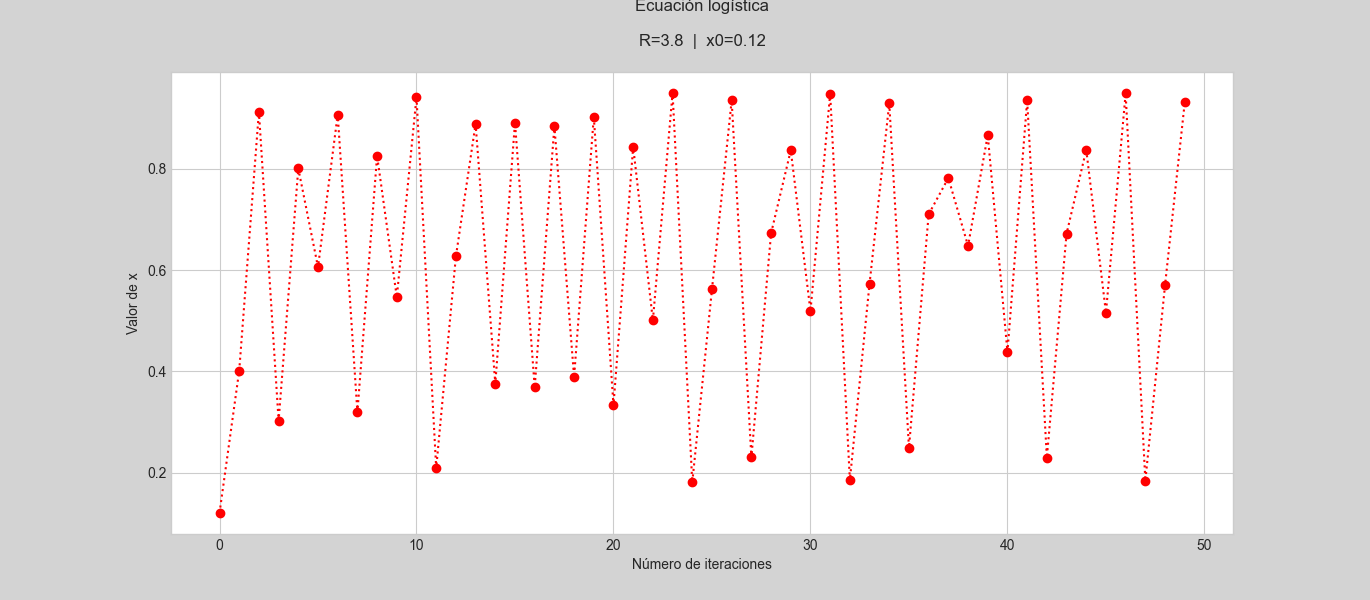
\includegraphics[scale=0.5]{Graf_5.png} 

\end{itemize}

Ahora queremos graficar los resultados de la "ecuación logística" para miles de valores diferente de $r$ (entre 2 y 4) en un diagrama. Para cada punto, haremos 500 iteraciones. Sólo graficaremos las primeras 100, y las primeras 400 serán una oportunidad para posible convergencia. El código empleado en el script \textit{Diagramasbifurcacion.py} se ve así,

\begin{python}
R_list = np.linspace(2.0, 4.0, 1000)
x0 = 0.3
N = 500

def logis(r):
    x_list = [x0]    
    for i in range(N-1):
        x_list.append(r * x_list[-1] * (1 - x_list[-1]))
    return x_list[400:]

x_select = []
R_select = []
for r in R_list:
    x_select.append(logis(r))
    R_select.append([r] * 100) 
    
x_select = np.array(x_select).ravel()
R_select = np.array(R_select).ravel()

plt.style.use('seaborn-whitegrid')
plt.figure(figsize=(16, 6), facecolor='lightgray')
plt.xlabel('The value of R')
plt.ylabel('The value of x')
plt.title(f'\nThe bifurcation diagram of the Logistic Equation\n\n2.0 < R < 4.0  |  x0=0.3\n')
plt.scatter(R_select, x_select, color='red', s=0.1)
plt.savefig('bifurcation_diagram.png')
plt.show()
\end{python}



\section{Creación de una base de datos}

	\subsection{Extracción de datos.}

		Para extraer los datos de los distintos índices económicos se empleó la API de YahooFinance, conocida como Yfinance. Se tomó esta decisión porque la mayoría de las API's con las mismas funciones eran de paga, y, por otro lado, era más fácil obtener los datos de esta manera que extrayendo los datos de forma directa aplicando técnicas de Web Scrapping. \\
		
		El uso de Yfinance es bastante simple, aún así creo esclarecedor una breve explicación de su funcionamiento. Yfinance se basa en un sistema de Tickets que son la forma de comunicarnos con el sitio Web de Yahoo Finance. Para emplear los tickets necesitamos de la clave con la que están designados los índices económicos, la cual puede ser consultada desde la página de YahooFinance. Por ejemplo, la clave del IPC MEXICO es "\^{}MXX". \\
		
		Con el ticket podemos consultar información del índice económico como sus acciones, sus dividendos, sus ganancias, etcétera. A continuación presentamos un ejemplo de código para consultar la información relacionada a un índice económico. \\
		
\begin{python}
import yfinance as yf
IPC = yf.Ticker("^MXX")
# Muestra acciones (dividendos, splits)		
IPC.actions 
# Muestra dividendos
IPC.dividens
# Muestra splits
IPC.splits
# Existen mas metodos, que pueden ser consultados en la documentacion
\end{python}

	Ahora con la posibilidad de obtener la información, necesitamos guardarla de algún modo. Y queríamos que fuera lo antes posible porque los datos con granularidad menor a un día en las series de tiempo se eliminaban después de 7 días. \\
	
	La solución fue que mientras se diseñaba la base de datos, los datos se almacenaran en formato ".csv". Para ello hice un script que almacenaba los datos en la computadora y que se activaba de forma automática todos los días. Ahora comentaré las partes de dicho código, y explicaré la forma en que lo automaticé.\\
	
	La primera parte del código es la importación de las funciones y librerias que ocuparemos, a saber;
	
	\begin{python}
import yfinance as yf
from pathlib import Path
from datetime import date, timedelta, datetime
import time
	\end{python}
		
	El módulo \pythoninline{pathlib} nos permite manipular las rutas de los archivos del sistema, de forma muy similar a \pythoninline{os.path}, pero con la diferencia de \pythoninline{pathlib} lo puede lograr a alto nivel y que su interface es mucho más conveniente. Por otro lado, los módulos \pythoninline{datetime} y \pythoninline{time} nos permite trabajar con fechas y tiempos, para ello emplea una clase conocida como datetime. \\
	
	La siguiente parte del código consiste en la enumeración de los tickets de los distintos índices económicos de los que queremos extraer la información. Como explicamos antes, para poder usar los tickets necesitamos el TAG de los ínidces económicos que aparecen en la página de YahooFinance. Así, por ejemplo, tenemos que el TAG del NASDAQ es "\^{}NDX"   ó del DOWJONES es " \^{}DJI". \\ 
	
	\begin{python}
SP500 = yf.Ticker("^GSPC") #S&P 500
Nasdaq =yf.Ticker("^NDX") #Nasdaq 100
Nasdaqcomp = yf.Ticker("^IXIC") #Nasdaq Composite
DWJ = yf.Ticker("^DJI") #Dow Jones Industrial Average
IPC = yf.Ticker('^MXX') #IPC (BMV)
STOXX50E = yf.Ticker('^STOXX50E') #STOXX50
Nikkei = yf.Ticker('^N225') #Nikkei
CSI300 = yf.Ticker('000300.SS') #CS1300	
	\end{python}  
	
	La siguiente parte del código comienza guardando en listas los tickets y el nombre de los mismos, esto lo hacemos así para usarlos en los ciclos tipo \pythoninline{for}.\\
	
	En el primer \pythoninline{for} establecemos las fechas usando el módulo \pythoninline{datetime}. El método \pythoninline{.today()} sirve, como se podría adivinar, para devolver la fecha del día de hoy en formato datetime. Por otro lado, el método \pythoninline{.replace()} sirve para modificar los valores de los datos tipo datetime. Y, la función \pythoninline{timedelta()} se usa para restar la cantidad de tiempo que se especifique.\\
	
	Así lo que estamos haciendo es obtener la fecha de hoy hasta siete días antes, en un intervalo de 23 horas. Estos serán los días que obtendremos la información de los tickets. \\
	
	En el siguiente \pythoninline{for}, que recorre la longitud de la lista de tickets, con el método \pythoninline{.history} obtenemos el historial de los tickets con intervalos de un minuto. Luego, con la función \pythoninline{Path} del módulo \pythoninline{pathlib} creamos con una ruta de acceso para los archivos .csv de acuerdo con el nombre del ticket y la fecha a la que pertenece, para ello usamos el método \pythoninline{.format}.\\
	
	Por último, con el método \pythoninline{.to_csv} convertimos el historiald de los tickets en .csv, y especificamos que deseamos los encabezados y los índices, de igual modo, especificamos la ruta en la que se guardará con el "filepath" que habíamos crado anteriormente. \\ 
	
	\begin{python}
tickets = [SP500, Nasdaq, Nasdaqcomp, DWJ, IPC, STOXX50E, Nikkei, CSI300]
ticketsname = ["SP500", "Nasdaq", "Nasdaqcomp", "DWJ", "IPC", "STOXX50", "Nikkei", "CSI300"]

for i in range(7):
    start = datetime.today().replace(hour = 0, minute = 0, second = 0 ) - timedelta(days= i +1)
    end = datetime.today().replace(hour = 23) - timedelta(days = i +1)

    for i in range(len(tickets)):
        historial = tickets[i].history(start=start, end=end , interval="1m") 
        filepath = Path('Info/{almacenamiento}/{name}_{date}.csv'
        	.format(almacenamiento = ticketsname[i] ,name = ticketsname[i], date = start.strftime('%Y-%m-%d')))
        filepath.parent.mkdir(parents=True, exist_ok=True)
        historial.to_csv(filepath, header=True, index=True)	
	\end{python}	
	
	Por otro lado para la automatización del script ocupé el administrador de tareas de windows. Para ello se crea un archivo .bat con la ruta en la que está guardada el ejecutable de python y el script. 
	
		\subsection{Diseño, implementación y automatización de la base de datos}
	
	El plan original era usar PostgresSQL como el sistema de gestión de base de datos, pero por cuestiones técnicas terminé usando MySQL. En fin, la implementación de la base de datos en SQL tiene el siguiente código, 
	
	
		
	
	
	
\section{Análisis de distintos índices}
	
	\subsection{Análisis general de los índices económicos}	
	
	
	\subsection{Análisis sobre complejidad de los índices económicos}
	
	Para el análisis sobre la entropía haremos uso del módulo \pythoninline{EntropyHub}, cuyo manula puede ser consultado \href{https://github.com/MattWillFlood/EntropyHub/blob/main/EntropyHub%20Guide.pdf}{\textbf{aquí}}.
	
	\subsubsection{Approximate entropy}
	
	El objetivo de la \textit{approximate entropy} (ApEn) es estimar la 
	
	\subsubsection{Sample entropy}
		
\section{Bibliografía}

	\url{https://algotrading101.com/learn/yfinance-guide/}
	
	\url{https://www.ncbi.nlm.nih.gov/pmc/articles/PMC7515030/}
	


\end{document}